\documentclass[1p]{elsarticle_modified}
%\bibliographystyle{elsarticle-num}

%\usepackage[colorlinks]{hyperref}
%\usepackage{abbrmath_seonhwa} %\Abb, \Ascr, \Acal ,\Abf, \Afrak
\usepackage{amsfonts}
\usepackage{amssymb}
\usepackage{amsmath}
\usepackage{amsthm}
\usepackage{scalefnt}
\usepackage{amsbsy}
\usepackage{kotex}
\usepackage{caption}
\usepackage{subfig}
\usepackage{color}
\usepackage{graphicx}
\usepackage{xcolor} %% white, black, red, green, blue, cyan, magenta, yellow
\usepackage{float}
\usepackage{setspace}
\usepackage{hyperref}

\usepackage{tikz}
\usetikzlibrary{arrows}

\usepackage{multirow}
\usepackage{array} % fixed length table
\usepackage{hhline}

%%%%%%%%%%%%%%%%%%%%%
\makeatletter
\renewcommand*\env@matrix[1][\arraystretch]{%
	\edef\arraystretch{#1}%
	\hskip -\arraycolsep
	\let\@ifnextchar\new@ifnextchar
	\array{*\c@MaxMatrixCols c}}
\makeatother %https://tex.stackexchange.com/questions/14071/how-can-i-increase-the-line-spacing-in-a-matrix
%%%%%%%%%%%%%%%

\usepackage[normalem]{ulem}

\newcommand{\msout}[1]{\ifmmode\text{\sout{\ensuremath{#1}}}\else\sout{#1}\fi}
%SOURCE: \msout is \stkout macro in https://tex.stackexchange.com/questions/20609/strikeout-in-math-mode

\newcommand{\cancel}[1]{
	\ifmmode
	{\color{red}\msout{#1}}
	\else
	{\color{red}\sout{#1}}
	\fi
}

\newcommand{\add}[1]{
	{\color{blue}\uwave{#1}}
}

\newcommand{\replace}[2]{
	\ifmmode
	{\color{red}\msout{#1}}{\color{blue}\uwave{#2}}
	\else
	{\color{red}\sout{#1}}{\color{blue}\uwave{#2}}
	\fi
}

\newcommand{\Sol}{\mathcal{S}} %segment
\newcommand{\D}{D} %diagram
\newcommand{\A}{\mathcal{A}} %arc


%%%%%%%%%%%%%%%%%%%%%%%%%%%%%5 test

\def\sl{\operatorname{\textup{SL}}(2,\Cbb)}
\def\psl{\operatorname{\textup{PSL}}(2,\Cbb)}
\def\quan{\mkern 1mu \triangleright \mkern 1mu}

\theoremstyle{definition}
\newtheorem{thm}{Theorem}[section]
\newtheorem{prop}[thm]{Proposition}
\newtheorem{lem}[thm]{Lemma}
\newtheorem{ques}[thm]{Question}
\newtheorem{cor}[thm]{Corollary}
\newtheorem{defn}[thm]{Definition}
\newtheorem{exam}[thm]{Example}
\newtheorem{rmk}[thm]{Remark}
\newtheorem{alg}[thm]{Algorithm}

\newcommand{\I}{\sqrt{-1}}
\begin{document}

%\begin{frontmatter}
%
%\title{Boundary parabolic representations of knots up to 8 crossings}
%
%%% Group authors per affiliation:
%\author{Yunhi Cho} 
%\address{Department of Mathematics, University of Seoul, Seoul, Korea}
%\ead{yhcho@uos.ac.kr}
%
%
%\author{Seonhwa Kim} %\fnref{s_kim}}
%\address{Center for Geometry and Physics, Institute for Basic Science, Pohang, 37673, Korea}
%\ead{ryeona17@ibs.re.kr}
%
%\author{Hyuk Kim}
%\address{Department of Mathematical Sciences, Seoul National University, Seoul 08826, Korea}
%\ead{hyukkim@snu.ac.kr}
%
%\author{Seokbeom Yoon}
%\address{Department of Mathematical Sciences, Seoul National University, Seoul, 08826,  Korea}
%\ead{sbyoon15@snu.ac.kr}
%
%\begin{abstract}
%We find all boundary parabolic representation of knots up to 8 crossings.
%
%\end{abstract}
%\begin{keyword}
%    \MSC[2010] 57M25 
%\end{keyword}
%
%\end{frontmatter}

%\linenumbers
%\tableofcontents
%
\newcommand\colored[1]{\textcolor{white}{\rule[-0.35ex]{0.8em}{1.4ex}}\kern-0.8em\color{red} #1}%
%\newcommand\colored[1]{\textcolor{white}{ #1}\kern-2.17ex	\textcolor{white}{ #1}\kern-1.81ex	\textcolor{white}{ #1}\kern-2.15ex\color{red}#1	}

{\Large $\underline{12a_{0021}~(K12a_{0021})}$}

\setlength{\tabcolsep}{10pt}
\renewcommand{\arraystretch}{1.6}
\vspace{1cm}\begin{tabular}{m{100pt}>{\centering\arraybackslash}m{274pt}}
\multirow{5}{120pt}{
	\centering
	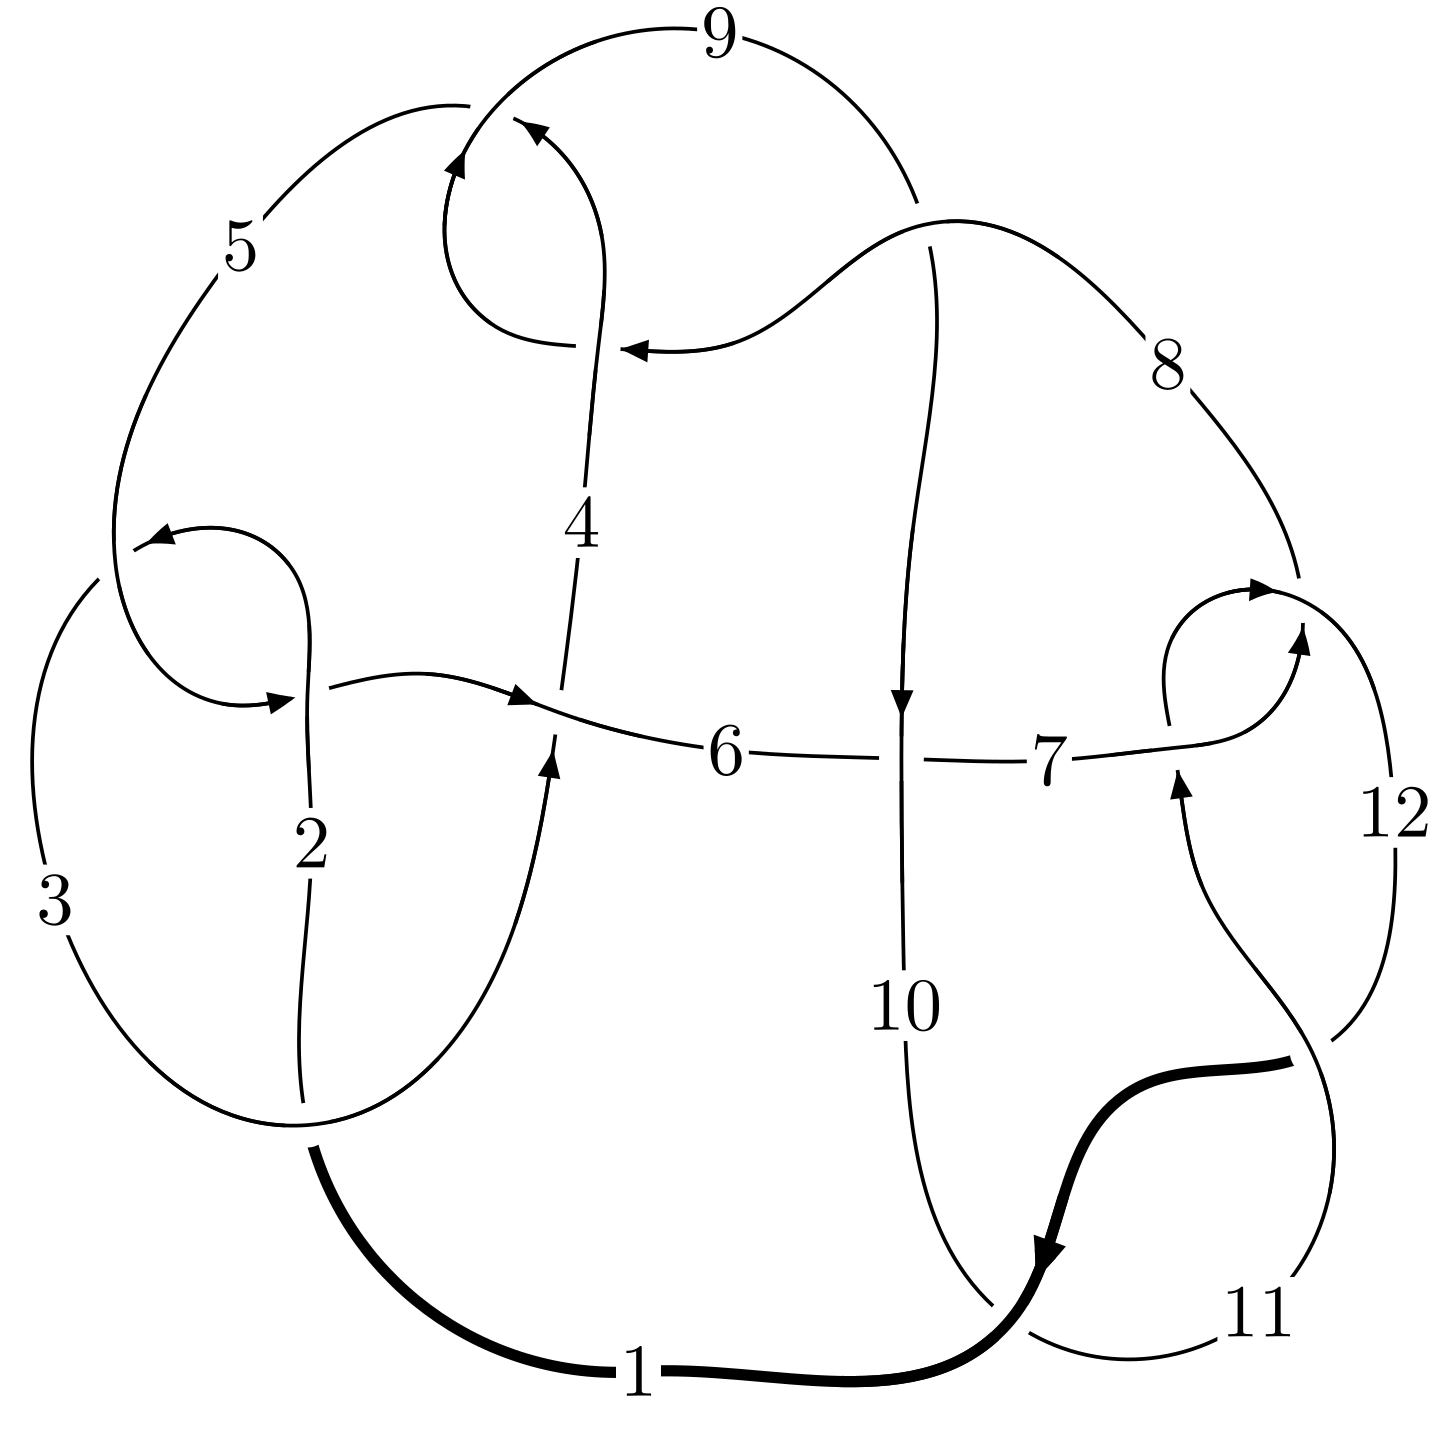
\includegraphics[width=112pt]{../../../GIT/diagram.site/Diagrams/png/822_12a_0021.png}\\
\ \ \ A knot diagram\footnotemark}&
\allowdisplaybreaks
\textbf{Linearized knot diagam} \\
\cline{2-2}
 &
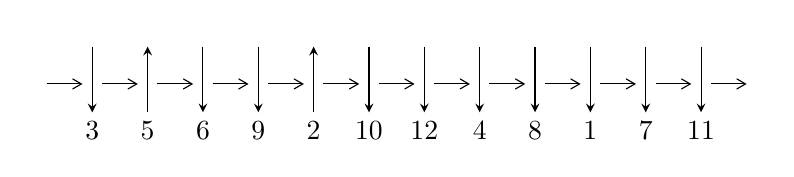
\begin{tikzpicture}[x=20pt, y=17pt]
	% nodes
	\node (C0) at (0, 0) {};
	\node (C1) at (1, 0) {};
	\node (C1U) at (1, +1) {};
	\node (C1D) at (1, -1) {3};

	\node (C2) at (2, 0) {};
	\node (C2U) at (2, +1) {};
	\node (C2D) at (2, -1) {5};

	\node (C3) at (3, 0) {};
	\node (C3U) at (3, +1) {};
	\node (C3D) at (3, -1) {6};

	\node (C4) at (4, 0) {};
	\node (C4U) at (4, +1) {};
	\node (C4D) at (4, -1) {9};

	\node (C5) at (5, 0) {};
	\node (C5U) at (5, +1) {};
	\node (C5D) at (5, -1) {2};

	\node (C6) at (6, 0) {};
	\node (C6U) at (6, +1) {};
	\node (C6D) at (6, -1) {10};

	\node (C7) at (7, 0) {};
	\node (C7U) at (7, +1) {};
	\node (C7D) at (7, -1) {12};

	\node (C8) at (8, 0) {};
	\node (C8U) at (8, +1) {};
	\node (C8D) at (8, -1) {4};

	\node (C9) at (9, 0) {};
	\node (C9U) at (9, +1) {};
	\node (C9D) at (9, -1) {8};

	\node (C10) at (10, 0) {};
	\node (C10U) at (10, +1) {};
	\node (C10D) at (10, -1) {1};

	\node (C11) at (11, 0) {};
	\node (C11U) at (11, +1) {};
	\node (C11D) at (11, -1) {7};

	\node (C12) at (12, 0) {};
	\node (C12U) at (12, +1) {};
	\node (C12D) at (12, -1) {11};
	\node (C13) at (13, 0) {};

	% arrows
	\draw[->,>={angle 60}]
	(C0) edge (C1) (C1) edge (C2) (C2) edge (C3) (C3) edge (C4) (C4) edge (C5) (C5) edge (C6) (C6) edge (C7) (C7) edge (C8) (C8) edge (C9) (C9) edge (C10) (C10) edge (C11) (C11) edge (C12) (C12) edge (C13) ;	\draw[->,>=stealth]
	(C1U) edge (C1D) (C2D) edge (C2U) (C3U) edge (C3D) (C4U) edge (C4D) (C5D) edge (C5U) (C6U) edge (C6D) (C7U) edge (C7D) (C8U) edge (C8D) (C9U) edge (C9D) (C10U) edge (C10D) (C11U) edge (C11D) (C12U) edge (C12D) ;
	\end{tikzpicture} \\
\hhline{~~} \\& 
\textbf{Solving Sequence} \\ \cline{2-2} 
 &
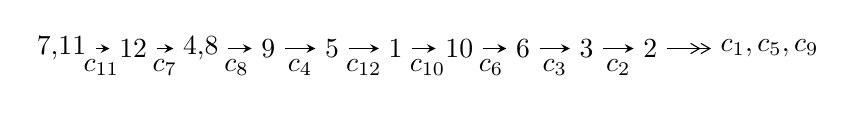
\begin{tikzpicture}[x=23pt, y=7pt]
	% node
	\node (A0) at (-1/8, 0) {7,11};
	\node (A1) at (1, 0) {12};
	\node (A2) at (33/16, 0) {4,8};
	\node (A3) at (25/8, 0) {9};
	\node (A4) at (33/8, 0) {5};
	\node (A5) at (41/8, 0) {1};
	\node (A6) at (49/8, 0) {10};
	\node (A7) at (57/8, 0) {6};
	\node (A8) at (65/8, 0) {3};
	\node (A9) at (73/8, 0) {2};
	\node (C1) at (1/2, -1) {$c_{11}$};
	\node (C2) at (3/2, -1) {$c_{7}$};
	\node (C3) at (21/8, -1) {$c_{8}$};
	\node (C4) at (29/8, -1) {$c_{4}$};
	\node (C5) at (37/8, -1) {$c_{12}$};
	\node (C6) at (45/8, -1) {$c_{10}$};
	\node (C7) at (53/8, -1) {$c_{6}$};
	\node (C8) at (61/8, -1) {$c_{3}$};
	\node (C9) at (69/8, -1) {$c_{2}$};
	\node (A10) at (11, 0) {$c_{1},c_{5},c_{9}$};

	% edge
	\draw[->,>=stealth]	
	(A0) edge (A1) (A1) edge (A2) (A2) edge (A3) (A3) edge (A4) (A4) edge (A5) (A5) edge (A6) (A6) edge (A7) (A7) edge (A8) (A8) edge (A9) ;
	\draw[->>,>={angle 60}]	
	(A9) edge (A10);
\end{tikzpicture} \\ 

\end{tabular} \\

\footnotetext{
The image of knot diagram is generated by the software ``\textbf{Draw programme}" developed by Andrew Bartholomew(\url{http://www.layer8.co.uk/maths/draw/index.htm\#Running-draw}), where we modified some parts for our purpose(\url{https://github.com/CATsTAILs/LinksPainter}).
}\phantom \\ \newline 
\centering \textbf{Ideals for irreducible components\footnotemark of $X_{\text{par}}$} 
 
\begin{align*}
I^u_{1}&=\langle 
-19 u^{103}-49 u^{102}+\cdots+2 b+19,\;-2 u^{103}+5 u^{102}+\cdots+2 a-6,\;u^{104}+3 u^{103}+\cdots- u-1\rangle \\
I^u_{2}&=\langle 
- u^2 a+b+a,\;u^2 a+a^2- a u- u+1,\;u^3- u^2+1\rangle \\
\\
\end{align*}
\raggedright * 2 irreducible components of $\dim_{\mathbb{C}}=0$, with total 110 representations.\\
\footnotetext{All coefficients of polynomials are rational numbers. But the coefficients are sometimes approximated in decimal forms when there is not enough margin.}
\newpage
\renewcommand{\arraystretch}{1}
\centering \section*{I. $I^u_{1}= \langle -19 u^{103}-49 u^{102}+\cdots+2 b+19,\;-2 u^{103}+5 u^{102}+\cdots+2 a-6,\;u^{104}+3 u^{103}+\cdots- u-1 \rangle$}
\flushleft \textbf{(i) Arc colorings}\\
\begin{tabular}{m{7pt} m{180pt} m{7pt} m{180pt} }
\flushright $a_{7}=$&$\begin{pmatrix}0\\u\end{pmatrix}$ \\
\flushright $a_{11}=$&$\begin{pmatrix}1\\0\end{pmatrix}$ \\
\flushright $a_{12}=$&$\begin{pmatrix}1\\u^2\end{pmatrix}$ \\
\flushright $a_{4}=$&$\begin{pmatrix}u^{103}-\frac{5}{2} u^{102}+\cdots-\frac{1}{2} u+3\\\frac{19}{2} u^{103}+\frac{49}{2} u^{102}+\cdots-4 u-\frac{19}{2}\end{pmatrix}$ \\
\flushright $a_{8}=$&$\begin{pmatrix}- u\\- u^3+u\end{pmatrix}$ \\
\flushright $a_{9}=$&$\begin{pmatrix}- u^8+u^6- u^4+1\\- u^{10}+2 u^8-3 u^6+2 u^4- u^2\end{pmatrix}$ \\
\flushright $a_{5}=$&$\begin{pmatrix}-2 u^{103}-\frac{23}{2} u^{102}+\cdots+\frac{1}{2} u+7\\\frac{23}{2} u^{103}+\frac{57}{2} u^{102}+\cdots-5 u-\frac{23}{2}\end{pmatrix}$ \\
\flushright $a_{1}=$&$\begin{pmatrix}- u^2+1\\u^2\end{pmatrix}$ \\
\flushright $a_{10}=$&$\begin{pmatrix}u^4- u^2+1\\- u^4\end{pmatrix}$ \\
\flushright $a_{6}=$&$\begin{pmatrix}u^9-2 u^7+3 u^5-2 u^3+u\\- u^9+u^7- u^5+u\end{pmatrix}$ \\
\flushright $a_{3}=$&$\begin{pmatrix}-5 u^{102}-\frac{13}{2} u^{101}+\cdots-\frac{1}{2} u+\frac{9}{2}\\9 u^{103}+23 u^{102}+\cdots-3 u-9\end{pmatrix}$ \\
\flushright $a_{2}=$&$\begin{pmatrix}- u^{102}-\frac{3}{2} u^{101}+\cdots+\frac{7}{2} u+\frac{5}{2}\\u^{103}+3 u^{102}+\cdots- u-1\end{pmatrix}$\\&\end{tabular}
\flushleft \textbf{(ii) Obstruction class $= -1$}\\~\\
\flushleft \textbf{(iii) Cusp Shapes $= \frac{33}{2} u^{103}+31 u^{102}+\cdots-\frac{1}{2} u-\frac{33}{2}$}\\~\\
\newpage\renewcommand{\arraystretch}{1}
\flushleft \textbf{(iv) u-Polynomials at the component}\newline \\
\begin{tabular}{m{50pt}|m{274pt}}
Crossings & \hspace{64pt}u-Polynomials at each crossing \\
\hline $$\begin{aligned}c_{1}\end{aligned}$$&$\begin{aligned}
&u^{104}+48 u^{103}+\cdots-24 u+1
\end{aligned}$\\
\hline $$\begin{aligned}c_{2},c_{5}\end{aligned}$$&$\begin{aligned}
&u^{104}+4 u^{103}+\cdots+8 u+1
\end{aligned}$\\
\hline $$\begin{aligned}c_{3}\end{aligned}$$&$\begin{aligned}
&u^{104}-4 u^{103}+\cdots-644 u+193
\end{aligned}$\\
\hline $$\begin{aligned}c_{4},c_{8}\end{aligned}$$&$\begin{aligned}
&u^{104}- u^{103}+\cdots-96 u-64
\end{aligned}$\\
\hline $$\begin{aligned}c_{6}\end{aligned}$$&$\begin{aligned}
&u^{104}-3 u^{103}+\cdots+14175 u-2425
\end{aligned}$\\
\hline $$\begin{aligned}c_{7},c_{11}\end{aligned}$$&$\begin{aligned}
&u^{104}+3 u^{103}+\cdots- u-1
\end{aligned}$\\
\hline $$\begin{aligned}c_{9}\end{aligned}$$&$\begin{aligned}
&u^{104}+35 u^{103}+\cdots+82944 u+4096
\end{aligned}$\\
\hline $$\begin{aligned}c_{10},c_{12}\end{aligned}$$&$\begin{aligned}
&u^{104}+33 u^{103}+\cdots+11 u+1
\end{aligned}$\\
\hline
\end{tabular}\\~\\
\newpage\renewcommand{\arraystretch}{1}
\flushleft \textbf{(v) Riley Polynomials at the component}\newline \\
\begin{tabular}{m{50pt}|m{274pt}}
Crossings & \hspace{64pt}Riley Polynomials at each crossing \\
\hline $$\begin{aligned}c_{1}\end{aligned}$$&$\begin{aligned}
&y^{104}+20 y^{103}+\cdots-556 y+1
\end{aligned}$\\
\hline $$\begin{aligned}c_{2},c_{5}\end{aligned}$$&$\begin{aligned}
&y^{104}+48 y^{103}+\cdots-24 y+1
\end{aligned}$\\
\hline $$\begin{aligned}c_{3}\end{aligned}$$&$\begin{aligned}
&y^{104}-8 y^{103}+\cdots-3334440 y+37249
\end{aligned}$\\
\hline $$\begin{aligned}c_{4},c_{8}\end{aligned}$$&$\begin{aligned}
&y^{104}-35 y^{103}+\cdots-82944 y+4096
\end{aligned}$\\
\hline $$\begin{aligned}c_{6}\end{aligned}$$&$\begin{aligned}
&y^{104}+19 y^{103}+\cdots+127099125 y+5880625
\end{aligned}$\\
\hline $$\begin{aligned}c_{7},c_{11}\end{aligned}$$&$\begin{aligned}
&y^{104}-33 y^{103}+\cdots-11 y+1
\end{aligned}$\\
\hline $$\begin{aligned}c_{9}\end{aligned}$$&$\begin{aligned}
&y^{104}+57 y^{103}+\cdots-571473920 y+16777216
\end{aligned}$\\
\hline $$\begin{aligned}c_{10},c_{12}\end{aligned}$$&$\begin{aligned}
&y^{104}+79 y^{103}+\cdots+285 y+1
\end{aligned}$\\
\hline
\end{tabular}\\~\\
\newpage\flushleft \textbf{(vi) Complex Volumes and Cusp Shapes}
$$\begin{array}{c|c|c}  
\text{Solutions to }I^u_{1}& \I (\text{vol} + \sqrt{-1}CS) & \text{Cusp shape}\\
 \hline 
\begin{aligned}
u &= -0.995545 + 0.161097 I \\
a &= -0.512579 - 0.871788 I \\
b &= -0.644479 - 0.792496 I\end{aligned}
 & -1.83155 + 5.70406 I & \phantom{-0.000000 } 0 \\ \hline\begin{aligned}
u &= -0.995545 - 0.161097 I \\
a &= -0.512579 + 0.871788 I \\
b &= -0.644479 + 0.792496 I\end{aligned}
 & -1.83155 - 5.70406 I & \phantom{-0.000000 } 0 \\ \hline\begin{aligned}
u &= \phantom{-}0.970059 + 0.180479 I \\
a &= \phantom{-}0.99729 - 1.32904 I \\
b &= -0.558830 + 0.049258 I\end{aligned}
 & -0.10724 - 3.95678 I & \phantom{-0.000000 } 0 \\ \hline\begin{aligned}
u &= \phantom{-}0.970059 - 0.180479 I \\
a &= \phantom{-}0.99729 + 1.32904 I \\
b &= -0.558830 - 0.049258 I\end{aligned}
 & -0.10724 + 3.95678 I & \phantom{-0.000000 } 0 \\ \hline\begin{aligned}
u &= -0.923833 + 0.339721 I \\
a &= \phantom{-}0.616132 + 0.482403 I \\
b &= \phantom{-}0.806426 + 0.318937 I\end{aligned}
 & -0.284227 - 0.543049 I & \phantom{-0.000000 } 0 \\ \hline\begin{aligned}
u &= -0.923833 - 0.339721 I \\
a &= \phantom{-}0.616132 - 0.482403 I \\
b &= \phantom{-}0.806426 - 0.318937 I\end{aligned}
 & -0.284227 + 0.543049 I & \phantom{-0.000000 } 0 \\ \hline\begin{aligned}
u &= \phantom{-}0.827173 + 0.596410 I \\
a &= -0.79732 + 1.46815 I \\
b &= -0.261002 - 1.178970 I\end{aligned}
 & -0.064833 + 0.905297 I & \phantom{-0.000000 } 0 \\ \hline\begin{aligned}
u &= \phantom{-}0.827173 - 0.596410 I \\
a &= -0.79732 - 1.46815 I \\
b &= -0.261002 + 1.178970 I\end{aligned}
 & -0.064833 - 0.905297 I & \phantom{-0.000000 } 0 \\ \hline\begin{aligned}
u &= \phantom{-}1.02711\phantom{ +0.000000I} \\
a &= -0.774739\phantom{ +0.000000I} \\
b &= \phantom{-}1.02521\phantom{ +0.000000I}\end{aligned}
 & -5.59162\phantom{ +0.000000I} & \phantom{-0.000000 } 0 \\ \hline\begin{aligned}
u &= -0.953515 + 0.186747 I \\
a &= \phantom{-}0.516727 + 0.739793 I \\
b &= \phantom{-}0.632602 + 0.622967 I\end{aligned}
 & \phantom{-}0.020107 + 1.034370 I & \phantom{-0.000000 } 0\\
 \hline 
 \end{array}$$\newpage$$\begin{array}{c|c|c}  
\text{Solutions to }I^u_{1}& \I (\text{vol} + \sqrt{-1}CS) & \text{Cusp shape}\\
 \hline 
\begin{aligned}
u &= -0.953515 - 0.186747 I \\
a &= \phantom{-}0.516727 - 0.739793 I \\
b &= \phantom{-}0.632602 - 0.622967 I\end{aligned}
 & \phantom{-}0.020107 - 1.034370 I & \phantom{-0.000000 } 0 \\ \hline\begin{aligned}
u &= -0.963413 + 0.068510 I \\
a &= -0.217097 - 0.862505 I \\
b &= -0.268461 - 0.816848 I\end{aligned}
 & -3.56083 - 0.88582 I & \phantom{-0.000000 } 0 \\ \hline\begin{aligned}
u &= -0.963413 - 0.068510 I \\
a &= -0.217097 + 0.862505 I \\
b &= -0.268461 + 0.816848 I\end{aligned}
 & -3.56083 + 0.88582 I & \phantom{-0.000000 } 0 \\ \hline\begin{aligned}
u &= -0.972667 + 0.372254 I \\
a &= -0.705354 - 0.386489 I \\
b &= -0.874004 - 0.283310 I\end{aligned}
 & -2.41063 - 5.32876 I & \phantom{-0.000000 } 0 \\ \hline\begin{aligned}
u &= -0.972667 - 0.372254 I \\
a &= -0.705354 + 0.386489 I \\
b &= -0.874004 + 0.283310 I\end{aligned}
 & -2.41063 + 5.32876 I & \phantom{-0.000000 } 0 \\ \hline\begin{aligned}
u &= -0.929413 + 0.472446 I \\
a &= -0.399519 - 0.237173 I \\
b &= -0.832935 - 0.303200 I\end{aligned}
 & -4.34073 + 1.98932 I & \phantom{-0.000000 } 0 \\ \hline\begin{aligned}
u &= -0.929413 - 0.472446 I \\
a &= -0.399519 + 0.237173 I \\
b &= -0.832935 + 0.303200 I\end{aligned}
 & -4.34073 - 1.98932 I & \phantom{-0.000000 } 0 \\ \hline\begin{aligned}
u &= \phantom{-}1.044070 + 0.145718 I \\
a &= -0.609037 + 1.077920 I \\
b &= \phantom{-}0.727801 + 0.244738 I\end{aligned}
 & -6.19328 - 3.93028 I & \phantom{-0.000000 } 0 \\ \hline\begin{aligned}
u &= \phantom{-}1.044070 - 0.145718 I \\
a &= -0.609037 - 1.077920 I \\
b &= \phantom{-}0.727801 - 0.244738 I\end{aligned}
 & -6.19328 + 3.93028 I & \phantom{-0.000000 } 0 \\ \hline\begin{aligned}
u &= \phantom{-}1.040560 + 0.185605 I \\
a &= \phantom{-}0.63194 - 1.31168 I \\
b &= -0.542661 - 0.263709 I\end{aligned}
 & -1.35514 - 6.47708 I & \phantom{-0.000000 } 0\\
 \hline 
 \end{array}$$\newpage$$\begin{array}{c|c|c}  
\text{Solutions to }I^u_{1}& \I (\text{vol} + \sqrt{-1}CS) & \text{Cusp shape}\\
 \hline 
\begin{aligned}
u &= \phantom{-}1.040560 - 0.185605 I \\
a &= \phantom{-}0.63194 + 1.31168 I \\
b &= -0.542661 + 0.263709 I\end{aligned}
 & -1.35514 + 6.47708 I & \phantom{-0.000000 } 0 \\ \hline\begin{aligned}
u &= \phantom{-}1.058190 + 0.027517 I \\
a &= \phantom{-}0.523585 - 0.218830 I \\
b &= -1.070460 - 0.065154 I\end{aligned}
 & -8.85013 - 3.97317 I & \phantom{-0.000000 } 0 \\ \hline\begin{aligned}
u &= \phantom{-}1.058190 - 0.027517 I \\
a &= \phantom{-}0.523585 + 0.218830 I \\
b &= -1.070460 + 0.065154 I\end{aligned}
 & -8.85013 + 3.97317 I & \phantom{-0.000000 } 0 \\ \hline\begin{aligned}
u &= \phantom{-}0.754441 + 0.751915 I \\
a &= \phantom{-}0.14946 - 1.60978 I \\
b &= \phantom{-}0.80789 + 1.57405 I\end{aligned}
 & \phantom{-}1.81411 - 1.60183 I & \phantom{-0.000000 } 0 \\ \hline\begin{aligned}
u &= \phantom{-}0.754441 - 0.751915 I \\
a &= \phantom{-}0.14946 + 1.60978 I \\
b &= \phantom{-}0.80789 - 1.57405 I\end{aligned}
 & \phantom{-}1.81411 + 1.60183 I & \phantom{-0.000000 } 0 \\ \hline\begin{aligned}
u &= -0.696471 + 0.811179 I \\
a &= \phantom{-}1.72568 + 1.53879 I \\
b &= -0.10925 - 2.61448 I\end{aligned}
 & \phantom{-}0.25197 - 3.78803 I & \phantom{-0.000000 } 0 \\ \hline\begin{aligned}
u &= -0.696471 - 0.811179 I \\
a &= \phantom{-}1.72568 - 1.53879 I \\
b &= -0.10925 + 2.61448 I\end{aligned}
 & \phantom{-}0.25197 + 3.78803 I & \phantom{-0.000000 } 0 \\ \hline\begin{aligned}
u &= \phantom{-}0.917559 + 0.150661 I \\
a &= -1.33133 + 1.31447 I \\
b &= \phantom{-}0.699472 - 0.238599 I\end{aligned}
 & -1.12265 + 1.04672 I & \phantom{-0.000000 } 0 \\ \hline\begin{aligned}
u &= \phantom{-}0.917559 - 0.150661 I \\
a &= -1.33133 - 1.31447 I \\
b &= \phantom{-}0.699472 + 0.238599 I\end{aligned}
 & -1.12265 - 1.04672 I & \phantom{-0.000000 } 0 \\ \hline\begin{aligned}
u &= -0.845342 + 0.657177 I \\
a &= -0.60933 + 1.32456 I \\
b &= \phantom{-}2.39972 + 0.27164 I\end{aligned}
 & \phantom{-}1.80047 + 0.06644 I & \phantom{-0.000000 } 0\\
 \hline 
 \end{array}$$\newpage$$\begin{array}{c|c|c}  
\text{Solutions to }I^u_{1}& \I (\text{vol} + \sqrt{-1}CS) & \text{Cusp shape}\\
 \hline 
\begin{aligned}
u &= -0.845342 - 0.657177 I \\
a &= -0.60933 - 1.32456 I \\
b &= \phantom{-}2.39972 - 0.27164 I\end{aligned}
 & \phantom{-}1.80047 - 0.06644 I & \phantom{-0.000000 } 0 \\ \hline\begin{aligned}
u &= \phantom{-}1.059270 + 0.187963 I \\
a &= -0.52976 + 1.33230 I \\
b &= \phantom{-}0.543826 + 0.360359 I\end{aligned}
 & -3.56774 - 11.61460 I & \phantom{-0.000000 } 0 \\ \hline\begin{aligned}
u &= \phantom{-}1.059270 - 0.187963 I \\
a &= -0.52976 - 1.33230 I \\
b &= \phantom{-}0.543826 - 0.360359 I\end{aligned}
 & -3.56774 + 11.61460 I & \phantom{-0.000000 } 0 \\ \hline\begin{aligned}
u &= \phantom{-}0.724424 + 0.808314 I \\
a &= \phantom{-}0.06007 - 1.91766 I \\
b &= \phantom{-}1.10628 + 2.12037 I\end{aligned}
 & \phantom{-}4.56534 + 5.10375 I & \phantom{-0.000000 } 0 \\ \hline\begin{aligned}
u &= \phantom{-}0.724424 - 0.808314 I \\
a &= \phantom{-}0.06007 + 1.91766 I \\
b &= \phantom{-}1.10628 - 2.12037 I\end{aligned}
 & \phantom{-}4.56534 - 5.10375 I & \phantom{-0.000000 } 0 \\ \hline\begin{aligned}
u &= -0.580019 + 0.700208 I \\
a &= -1.098130 - 0.872380 I \\
b &= -0.018720 + 0.778011 I\end{aligned}
 & -3.49153 - 4.75928 I & \phantom{-0.000000 } 0 \\ \hline\begin{aligned}
u &= -0.580019 - 0.700208 I \\
a &= -1.098130 + 0.872380 I \\
b &= -0.018720 - 0.778011 I\end{aligned}
 & -3.49153 + 4.75928 I & \phantom{-0.000000 } 0 \\ \hline\begin{aligned}
u &= -0.749031 + 0.797955 I \\
a &= \phantom{-}1.63183 + 2.03735 I \\
b &= \phantom{-}0.75933 - 3.15840 I\end{aligned}
 & \phantom{-}5.02616 + 2.15983 I & \phantom{-0.000000 } 0 \\ \hline\begin{aligned}
u &= -0.749031 - 0.797955 I \\
a &= \phantom{-}1.63183 - 2.03735 I \\
b &= \phantom{-}0.75933 + 3.15840 I\end{aligned}
 & \phantom{-}5.02616 - 2.15983 I & \phantom{-0.000000 } 0 \\ \hline\begin{aligned}
u &= -0.736317 + 0.810407 I \\
a &= -1.75080 - 1.89744 I \\
b &= -0.39215 + 3.15606 I\end{aligned}
 & \phantom{-}6.34017 - 3.11840 I & \phantom{-0.000000 } 0\\
 \hline 
 \end{array}$$\newpage$$\begin{array}{c|c|c}  
\text{Solutions to }I^u_{1}& \I (\text{vol} + \sqrt{-1}CS) & \text{Cusp shape}\\
 \hline 
\begin{aligned}
u &= -0.736317 - 0.810407 I \\
a &= -1.75080 + 1.89744 I \\
b &= -0.39215 - 3.15606 I\end{aligned}
 & \phantom{-}6.34017 + 3.11840 I & \phantom{-0.000000 } 0 \\ \hline\begin{aligned}
u &= -0.712069 + 0.832469 I \\
a &= -1.92411 - 1.64609 I \\
b &= \phantom{-}0.23828 + 3.07167 I\end{aligned}
 & \phantom{-}5.42558 - 6.12943 I & \phantom{-0.000000 } 0 \\ \hline\begin{aligned}
u &= -0.712069 - 0.832469 I \\
a &= -1.92411 + 1.64609 I \\
b &= \phantom{-}0.23828 - 3.07167 I\end{aligned}
 & \phantom{-}5.42558 + 6.12943 I & \phantom{-0.000000 } 0 \\ \hline\begin{aligned}
u &= -0.705084 + 0.840871 I \\
a &= \phantom{-}1.98457 + 1.57228 I \\
b &= -0.44329 - 3.05691 I\end{aligned}
 & \phantom{-}3.32150 - 11.40490 I & \phantom{-0.000000 } 0 \\ \hline\begin{aligned}
u &= -0.705084 - 0.840871 I \\
a &= \phantom{-}1.98457 - 1.57228 I \\
b &= -0.44329 + 3.05691 I\end{aligned}
 & \phantom{-}3.32150 + 11.40490 I & \phantom{-0.000000 } 0 \\ \hline\begin{aligned}
u &= \phantom{-}0.863688 + 0.677581 I \\
a &= \phantom{-}0.706681 - 1.039710 I \\
b &= \phantom{-}0.260899 + 1.104450 I\end{aligned}
 & \phantom{-}2.19668 - 2.61840 I & \phantom{-0.000000 } 0 \\ \hline\begin{aligned}
u &= \phantom{-}0.863688 - 0.677581 I \\
a &= \phantom{-}0.706681 + 1.039710 I \\
b &= \phantom{-}0.260899 - 1.104450 I\end{aligned}
 & \phantom{-}2.19668 + 2.61840 I & \phantom{-0.000000 } 0 \\ \hline\begin{aligned}
u &= \phantom{-}0.742286 + 0.808762 I \\
a &= \phantom{-}0.02357 + 1.86766 I \\
b &= -1.23942 - 1.96405 I\end{aligned}
 & \phantom{-}6.44605 + 0.06854 I & \phantom{-0.000000 } 0 \\ \hline\begin{aligned}
u &= \phantom{-}0.742286 - 0.808762 I \\
a &= \phantom{-}0.02357 - 1.86766 I \\
b &= -1.23942 + 1.96405 I\end{aligned}
 & \phantom{-}6.44605 - 0.06854 I & \phantom{-0.000000 } 0 \\ \hline\begin{aligned}
u &= -0.886276 + 0.662580 I \\
a &= \phantom{-}1.19777 - 0.80402 I \\
b &= -2.29133 - 1.30899 I\end{aligned}
 & \phantom{-}1.66908 + 5.06000 I & \phantom{-0.000000 } 0\\
 \hline 
 \end{array}$$\newpage$$\begin{array}{c|c|c}  
\text{Solutions to }I^u_{1}& \I (\text{vol} + \sqrt{-1}CS) & \text{Cusp shape}\\
 \hline 
\begin{aligned}
u &= -0.886276 - 0.662580 I \\
a &= \phantom{-}1.19777 + 0.80402 I \\
b &= -2.29133 + 1.30899 I\end{aligned}
 & \phantom{-}1.66908 - 5.06000 I & \phantom{-0.000000 } 0 \\ \hline\begin{aligned}
u &= \phantom{-}0.919787 + 0.634859 I \\
a &= -1.14826 + 1.18703 I \\
b &= -0.297211 - 1.298160 I\end{aligned}
 & -0.40958 - 5.76100 I & \phantom{-0.000000 } 0 \\ \hline\begin{aligned}
u &= \phantom{-}0.919787 - 0.634859 I \\
a &= -1.14826 - 1.18703 I \\
b &= -0.297211 + 1.298160 I\end{aligned}
 & -0.40958 + 5.76100 I & \phantom{-0.000000 } 0 \\ \hline\begin{aligned}
u &= -0.628192 + 0.614774 I \\
a &= \phantom{-}0.802455 + 0.921266 I \\
b &= \phantom{-}0.543250 - 0.575702 I\end{aligned}
 & -0.763936 - 0.604697 I & \phantom{-0.000000 } 0 \\ \hline\begin{aligned}
u &= -0.628192 - 0.614774 I \\
a &= \phantom{-}0.802455 - 0.921266 I \\
b &= \phantom{-}0.543250 + 0.575702 I\end{aligned}
 & -0.763936 + 0.604697 I & \phantom{-0.000000 } 0 \\ \hline\begin{aligned}
u &= \phantom{-}0.780695 + 0.820092 I \\
a &= \phantom{-}0.27330 + 1.78142 I \\
b &= -1.61646 - 1.61478 I\end{aligned}
 & \phantom{-}6.65697 - 2.35527 I & \phantom{-0.000000 } 0 \\ \hline\begin{aligned}
u &= \phantom{-}0.780695 - 0.820092 I \\
a &= \phantom{-}0.27330 - 1.78142 I \\
b &= -1.61646 + 1.61478 I\end{aligned}
 & \phantom{-}6.65697 + 2.35527 I & \phantom{-0.000000 } 0 \\ \hline\begin{aligned}
u &= \phantom{-}0.795951 + 0.829057 I \\
a &= -0.41309 - 1.76927 I \\
b &= \phantom{-}1.83155 + 1.46562 I\end{aligned}
 & \phantom{-}4.94995 - 7.32695 I & \phantom{-0.000000 } 0 \\ \hline\begin{aligned}
u &= \phantom{-}0.795951 - 0.829057 I \\
a &= -0.41309 + 1.76927 I \\
b &= \phantom{-}1.83155 - 1.46562 I\end{aligned}
 & \phantom{-}4.94995 + 7.32695 I & \phantom{-0.000000 } 0 \\ \hline\begin{aligned}
u &= \phantom{-}0.852838 + 0.784493 I \\
a &= -0.518582 - 1.043630 I \\
b &= \phantom{-}1.299520 + 0.425878 I\end{aligned}
 & \phantom{-}2.51710 - 1.46458 I & \phantom{-0.000000 } 0\\
 \hline 
 \end{array}$$\newpage$$\begin{array}{c|c|c}  
\text{Solutions to }I^u_{1}& \I (\text{vol} + \sqrt{-1}CS) & \text{Cusp shape}\\
 \hline 
\begin{aligned}
u &= \phantom{-}0.852838 - 0.784493 I \\
a &= -0.518582 + 1.043630 I \\
b &= \phantom{-}1.299520 - 0.425878 I\end{aligned}
 & \phantom{-}2.51710 + 1.46458 I & \phantom{-0.000000 } 0 \\ \hline\begin{aligned}
u &= -0.987793 + 0.609954 I \\
a &= -0.282065 - 0.575521 I \\
b &= \phantom{-}0.324092 + 1.057970 I\end{aligned}
 & -5.36885 + 2.02799 I & \phantom{-0.000000 } 0 \\ \hline\begin{aligned}
u &= -0.987793 - 0.609954 I \\
a &= -0.282065 + 0.575521 I \\
b &= \phantom{-}0.324092 - 1.057970 I\end{aligned}
 & -5.36885 - 2.02799 I & \phantom{-0.000000 } 0 \\ \hline\begin{aligned}
u &= -0.977994 + 0.645453 I \\
a &= \phantom{-}0.727268 + 0.700582 I \\
b &= -0.32712 - 1.62271 I\end{aligned}
 & -1.73240 + 5.61848 I & \phantom{-0.000000 } 0 \\ \hline\begin{aligned}
u &= -0.977994 - 0.645453 I \\
a &= \phantom{-}0.727268 - 0.700582 I \\
b &= -0.32712 + 1.62271 I\end{aligned}
 & -1.73240 - 5.61848 I & \phantom{-0.000000 } 0 \\ \hline\begin{aligned}
u &= \phantom{-}0.903916 + 0.776679 I \\
a &= \phantom{-}1.058770 + 0.461633 I \\
b &= -1.179650 + 0.645136 I\end{aligned}
 & \phantom{-}2.36486 - 4.40594 I & \phantom{-0.000000 } 0 \\ \hline\begin{aligned}
u &= \phantom{-}0.903916 - 0.776679 I \\
a &= \phantom{-}1.058770 - 0.461633 I \\
b &= -1.179650 - 0.645136 I\end{aligned}
 & \phantom{-}2.36486 + 4.40594 I & \phantom{-0.000000 } 0 \\ \hline\begin{aligned}
u &= -1.004180 + 0.651392 I \\
a &= -0.581678 - 1.044430 I \\
b &= -0.15909 + 1.56067 I\end{aligned}
 & -4.68776 + 9.95104 I & \phantom{-0.000000 } 0 \\ \hline\begin{aligned}
u &= -1.004180 - 0.651392 I \\
a &= -0.581678 + 1.044430 I \\
b &= -0.15909 - 1.56067 I\end{aligned}
 & -4.68776 - 9.95104 I & \phantom{-0.000000 } 0 \\ \hline\begin{aligned}
u &= \phantom{-}0.966141 + 0.711656 I \\
a &= \phantom{-}1.60909 - 0.60969 I \\
b &= -0.20766 + 1.74080 I\end{aligned}
 & \phantom{-}1.16387 - 3.97141 I & \phantom{-0.000000 } 0\\
 \hline 
 \end{array}$$\newpage$$\begin{array}{c|c|c}  
\text{Solutions to }I^u_{1}& \I (\text{vol} + \sqrt{-1}CS) & \text{Cusp shape}\\
 \hline 
\begin{aligned}
u &= \phantom{-}0.966141 - 0.711656 I \\
a &= \phantom{-}1.60909 + 0.60969 I \\
b &= -0.20766 - 1.74080 I\end{aligned}
 & \phantom{-}1.16387 + 3.97141 I & \phantom{-0.000000 } 0 \\ \hline\begin{aligned}
u &= -0.977928 + 0.735033 I \\
a &= \phantom{-}1.85603 + 1.77296 I \\
b &= \phantom{-}0.58235 - 3.71912 I\end{aligned}
 & \phantom{-}4.32467 + 3.61431 I & \phantom{-0.000000 } 0 \\ \hline\begin{aligned}
u &= -0.977928 - 0.735033 I \\
a &= \phantom{-}1.85603 - 1.77296 I \\
b &= \phantom{-}0.58235 + 3.71912 I\end{aligned}
 & \phantom{-}4.32467 - 3.61431 I & \phantom{-0.000000 } 0 \\ \hline\begin{aligned}
u &= -0.463429 + 0.618913 I \\
a &= -0.886522 - 0.630657 I \\
b &= -0.149445 + 0.130543 I\end{aligned}
 & -4.04796 + 2.71125 I & -12.61990 - 3.98241 I \\ \hline\begin{aligned}
u &= -0.463429 - 0.618913 I \\
a &= -0.886522 + 0.630657 I \\
b &= -0.149445 - 0.130543 I\end{aligned}
 & -4.04796 - 2.71125 I & -12.61990 + 3.98241 I \\ \hline\begin{aligned}
u &= \phantom{-}0.966506 + 0.761778 I \\
a &= -1.80162 + 0.05991 I \\
b &= \phantom{-}0.94812 - 1.84887 I\end{aligned}
 & \phantom{-}6.08454 - 3.56908 I & \phantom{-0.000000 } 0 \\ \hline\begin{aligned}
u &= \phantom{-}0.966506 - 0.761778 I \\
a &= -1.80162 - 0.05991 I \\
b &= \phantom{-}0.94812 + 1.84887 I\end{aligned}
 & \phantom{-}6.08454 + 3.56908 I & \phantom{-0.000000 } 0 \\ \hline\begin{aligned}
u &= \phantom{-}0.985337 + 0.739108 I \\
a &= -1.90868 + 0.39757 I \\
b &= \phantom{-}0.51937 - 2.08817 I\end{aligned}
 & \phantom{-}5.70138 - 5.88628 I & \phantom{-0.000000 } 0 \\ \hline\begin{aligned}
u &= \phantom{-}0.985337 - 0.739108 I \\
a &= -1.90868 - 0.39757 I \\
b &= \phantom{-}0.51937 + 2.08817 I\end{aligned}
 & \phantom{-}5.70138 + 5.88628 I & \phantom{-0.000000 } 0 \\ \hline\begin{aligned}
u &= -0.989286 + 0.737835 I \\
a &= -1.70215 - 1.92426 I \\
b &= -0.90767 + 3.58230 I\end{aligned}
 & \phantom{-}5.56561 + 8.93649 I & \phantom{-0.000000 } 0\\
 \hline 
 \end{array}$$\newpage$$\begin{array}{c|c|c}  
\text{Solutions to }I^u_{1}& \I (\text{vol} + \sqrt{-1}CS) & \text{Cusp shape}\\
 \hline 
\begin{aligned}
u &= -0.989286 - 0.737835 I \\
a &= -1.70215 + 1.92426 I \\
b &= -0.90767 - 3.58230 I\end{aligned}
 & \phantom{-}5.56561 - 8.93649 I & \phantom{-0.000000 } 0 \\ \hline\begin{aligned}
u &= \phantom{-}0.960435 + 0.775381 I \\
a &= \phantom{-}1.79571 + 0.13146 I \\
b &= -1.20786 + 1.76111 I\end{aligned}
 & \phantom{-}4.44270 + 1.33279 I & \phantom{-0.000000 } 0 \\ \hline\begin{aligned}
u &= \phantom{-}0.960435 - 0.775381 I \\
a &= \phantom{-}1.79571 - 0.13146 I \\
b &= -1.20786 - 1.76111 I\end{aligned}
 & \phantom{-}4.44270 - 1.33279 I & \phantom{-0.000000 } 0 \\ \hline\begin{aligned}
u &= \phantom{-}0.994976 + 0.732633 I \\
a &= \phantom{-}1.97881 - 0.50784 I \\
b &= -0.37833 + 2.20105 I\end{aligned}
 & \phantom{-}3.73893 - 10.89850 I & \phantom{-0.000000 } 0 \\ \hline\begin{aligned}
u &= \phantom{-}0.994976 - 0.732633 I \\
a &= \phantom{-}1.97881 + 0.50784 I \\
b &= -0.37833 - 2.20105 I\end{aligned}
 & \phantom{-}3.73893 + 10.89850 I & \phantom{-0.000000 } 0 \\ \hline\begin{aligned}
u &= -1.009160 + 0.724746 I \\
a &= \phantom{-}1.29694 + 1.92384 I \\
b &= \phantom{-}1.13741 - 2.95407 I\end{aligned}
 & -0.69811 + 9.56220 I & \phantom{-0.000000 } 0 \\ \hline\begin{aligned}
u &= -1.009160 - 0.724746 I \\
a &= \phantom{-}1.29694 - 1.92384 I \\
b &= \phantom{-}1.13741 + 2.95407 I\end{aligned}
 & -0.69811 - 9.56220 I & \phantom{-0.000000 } 0 \\ \hline\begin{aligned}
u &= -1.010060 + 0.739826 I \\
a &= -1.42104 - 2.13601 I \\
b &= -1.40773 + 3.26557 I\end{aligned}
 & \phantom{-}4.51266 + 12.01460 I & \phantom{-0.000000 } 0 \\ \hline\begin{aligned}
u &= -1.010060 - 0.739826 I \\
a &= -1.42104 + 2.13601 I \\
b &= -1.40773 - 3.26557 I\end{aligned}
 & \phantom{-}4.51266 - 12.01460 I & \phantom{-0.000000 } 0 \\ \hline\begin{aligned}
u &= -1.016650 + 0.740942 I \\
a &= \phantom{-}1.34178 + 2.20727 I \\
b &= \phantom{-}1.56778 - 3.17605 I\end{aligned}
 & \phantom{-}2.3661 + 17.3165 I & \phantom{-0.000000 } 0\\
 \hline 
 \end{array}$$\newpage$$\begin{array}{c|c|c}  
\text{Solutions to }I^u_{1}& \I (\text{vol} + \sqrt{-1}CS) & \text{Cusp shape}\\
 \hline 
\begin{aligned}
u &= -1.016650 - 0.740942 I \\
a &= \phantom{-}1.34178 - 2.20727 I \\
b &= \phantom{-}1.56778 + 3.17605 I\end{aligned}
 & \phantom{-}2.3661 - 17.3165 I & \phantom{-0.000000 } 0 \\ \hline\begin{aligned}
u &= -0.112674 + 0.678362 I \\
a &= \phantom{-}0.254326 + 0.561225 I \\
b &= \phantom{-}0.929761 + 0.461434 I\end{aligned}
 & \phantom{-}0.24933 + 8.87552 I & -6.42415 - 7.58828 I \\ \hline\begin{aligned}
u &= -0.112674 - 0.678362 I \\
a &= \phantom{-}0.254326 - 0.561225 I \\
b &= \phantom{-}0.929761 - 0.461434 I\end{aligned}
 & \phantom{-}0.24933 - 8.87552 I & -6.42415 + 7.58828 I \\ \hline\begin{aligned}
u &= -0.095198 + 0.648369 I \\
a &= -0.257752 - 0.658833 I \\
b &= -0.939789 - 0.327643 I\end{aligned}
 & \phantom{-}2.30568 + 3.82799 I & -3.04052 - 3.48068 I \\ \hline\begin{aligned}
u &= -0.095198 - 0.648369 I \\
a &= -0.257752 + 0.658833 I \\
b &= -0.939789 + 0.327643 I\end{aligned}
 & \phantom{-}2.30568 - 3.82799 I & -3.04052 + 3.48068 I \\ \hline\begin{aligned}
u &= -0.180364 + 0.604663 I \\
a &= \phantom{-}0.495672 + 0.639352 I \\
b &= \phantom{-}0.642731 + 0.286163 I\end{aligned}
 & -2.31740 + 1.66077 I & -10.16858 - 2.73214 I \\ \hline\begin{aligned}
u &= -0.180364 - 0.604663 I \\
a &= \phantom{-}0.495672 - 0.639352 I \\
b &= \phantom{-}0.642731 - 0.286163 I\end{aligned}
 & -2.31740 - 1.66077 I & -10.16858 + 2.73214 I \\ \hline\begin{aligned}
u &= -0.598144\phantom{ +0.000000I} \\
a &= \phantom{-}0.647574\phantom{ +0.000000I} \\
b &= \phantom{-}0.367048\phantom{ +0.000000I}\end{aligned}
 & -0.843004\phantom{ +0.000000I} & -11.7650\phantom{ +0.000000I} \\ \hline\begin{aligned}
u &= -0.010244 + 0.579474 I \\
a &= -0.197590 - 0.954778 I \\
b &= -0.999928 + 0.022692 I\end{aligned}
 & \phantom{-}2.95584 + 1.48192 I & -1.41514 - 2.95992 I \\ \hline\begin{aligned}
u &= -0.010244 - 0.579474 I \\
a &= -0.197590 + 0.954778 I \\
b &= -0.999928 - 0.022692 I\end{aligned}
 & \phantom{-}2.95584 - 1.48192 I & -1.41514 + 2.95992 I\\
 \hline 
 \end{array}$$\newpage$$\begin{array}{c|c|c}  
\text{Solutions to }I^u_{1}& \I (\text{vol} + \sqrt{-1}CS) & \text{Cusp shape}\\
 \hline 
\begin{aligned}
u &= \phantom{-}0.056043 + 0.556970 I \\
a &= \phantom{-}0.110277 + 1.130210 I \\
b &= \phantom{-}1.034060 - 0.226304 I\end{aligned}
 & \phantom{-}1.46285 - 3.40463 I & -3.80359 + 2.83507 I \\ \hline\begin{aligned}
u &= \phantom{-}0.056043 - 0.556970 I \\
a &= \phantom{-}0.110277 - 1.130210 I \\
b &= \phantom{-}1.034060 + 0.226304 I\end{aligned}
 & \phantom{-}1.46285 + 3.40463 I & -3.80359 - 2.83507 I \\ \hline\begin{aligned}
u &= \phantom{-}0.213318 + 0.171099 I \\
a &= \phantom{-}0.30126 + 2.36442 I \\
b &= \phantom{-}0.286313 - 0.575206 I\end{aligned}
 & -0.33801 + 1.74815 I & -2.36854 - 3.15485 I \\ \hline\begin{aligned}
u &= \phantom{-}0.213318 - 0.171099 I \\
a &= \phantom{-}0.30126 - 2.36442 I \\
b &= \phantom{-}0.286313 + 0.575206 I\end{aligned}
 & -0.33801 - 1.74815 I & -2.36854 + 3.15485 I\\
 \hline 
 \end{array}$$\newpage\newpage\renewcommand{\arraystretch}{1}
\centering \section*{II. $I^u_{2}= \langle - u^2 a+b+a,\;u^2 a+a^2- a u- u+1,\;u^3- u^2+1 \rangle$}
\flushleft \textbf{(i) Arc colorings}\\
\begin{tabular}{m{7pt} m{180pt} m{7pt} m{180pt} }
\flushright $a_{7}=$&$\begin{pmatrix}0\\u\end{pmatrix}$ \\
\flushright $a_{11}=$&$\begin{pmatrix}1\\0\end{pmatrix}$ \\
\flushright $a_{12}=$&$\begin{pmatrix}1\\u^2\end{pmatrix}$ \\
\flushright $a_{4}=$&$\begin{pmatrix}a\\u^2 a- a\end{pmatrix}$ \\
\flushright $a_{8}=$&$\begin{pmatrix}- u\\- u^2+u+1\end{pmatrix}$ \\
\flushright $a_{9}=$&$\begin{pmatrix}- u\\- u^2+u+1\end{pmatrix}$ \\
\flushright $a_{5}=$&$\begin{pmatrix}a\\u^2 a- a\end{pmatrix}$ \\
\flushright $a_{1}=$&$\begin{pmatrix}- u^2+1\\u^2\end{pmatrix}$ \\
\flushright $a_{10}=$&$\begin{pmatrix}- u\\- u^2+u+1\end{pmatrix}$ \\
\flushright $a_{6}=$&$\begin{pmatrix}u^2-1\\- u^2\end{pmatrix}$ \\
\flushright $a_{3}=$&$\begin{pmatrix}- u^2 a+a u+2 a\\2 u^2 a-2 a\end{pmatrix}$ \\
\flushright $a_{2}=$&$\begin{pmatrix}- u^2 a+a u+u^2+2 a- u\\2 u^2 a- u^2-2 a\end{pmatrix}$\\&\end{tabular}
\flushleft \textbf{(ii) Obstruction class $= 1$}\\~\\
\flushleft \textbf{(iii) Cusp Shapes $= - u^2 a+6 a u- u^2+6 u-11$}\\~\\
\newpage\renewcommand{\arraystretch}{1}
\flushleft \textbf{(iv) u-Polynomials at the component}\newline \\
\begin{tabular}{m{50pt}|m{274pt}}
Crossings & \hspace{64pt}u-Polynomials at each crossing \\
\hline $$\begin{aligned}c_{1},c_{3},c_{5}\end{aligned}$$&$\begin{aligned}
&(u^2- u+1)^3
\end{aligned}$\\
\hline $$\begin{aligned}c_{2}\end{aligned}$$&$\begin{aligned}
&(u^2+u+1)^3
\end{aligned}$\\
\hline $$\begin{aligned}c_{4},c_{8},c_{9}\end{aligned}$$&$\begin{aligned}
&u^6
\end{aligned}$\\
\hline $$\begin{aligned}c_{6},c_{10}\end{aligned}$$&$\begin{aligned}
&(u^3- u^2+2 u-1)^2
\end{aligned}$\\
\hline $$\begin{aligned}c_{7}\end{aligned}$$&$\begin{aligned}
&(u^3+u^2-1)^2
\end{aligned}$\\
\hline $$\begin{aligned}c_{11}\end{aligned}$$&$\begin{aligned}
&(u^3- u^2+1)^2
\end{aligned}$\\
\hline $$\begin{aligned}c_{12}\end{aligned}$$&$\begin{aligned}
&(u^3+u^2+2 u+1)^2
\end{aligned}$\\
\hline
\end{tabular}\\~\\
\newpage\renewcommand{\arraystretch}{1}
\flushleft \textbf{(v) Riley Polynomials at the component}\newline \\
\begin{tabular}{m{50pt}|m{274pt}}
Crossings & \hspace{64pt}Riley Polynomials at each crossing \\
\hline $$\begin{aligned}c_{1},c_{2},c_{3}\\c_{5}\end{aligned}$$&$\begin{aligned}
&(y^2+y+1)^3
\end{aligned}$\\
\hline $$\begin{aligned}c_{4},c_{8},c_{9}\end{aligned}$$&$\begin{aligned}
&y^6
\end{aligned}$\\
\hline $$\begin{aligned}c_{6},c_{10},c_{12}\end{aligned}$$&$\begin{aligned}
&(y^3+3 y^2+2 y-1)^2
\end{aligned}$\\
\hline $$\begin{aligned}c_{7},c_{11}\end{aligned}$$&$\begin{aligned}
&(y^3- y^2+2 y-1)^2
\end{aligned}$\\
\hline
\end{tabular}\\~\\
\newpage\flushleft \textbf{(vi) Complex Volumes and Cusp Shapes}
$$\begin{array}{c|c|c}  
\text{Solutions to }I^u_{2}& \I (\text{vol} + \sqrt{-1}CS) & \text{Cusp shape}\\
 \hline 
\begin{aligned}
u &= \phantom{-}0.877439 + 0.744862 I \\
a &= \phantom{-}0.818128 + 0.292480 I \\
b &= -1.024480 + 0.839835 I\end{aligned}
 & \phantom{-}3.02413 - 0.79824 I & -4.03424 - 1.64667 I \\ \hline\begin{aligned}
u &= \phantom{-}0.877439 + 0.744862 I \\
a &= -0.155769 - 0.854759 I \\
b &= \phantom{-}1.239560 + 0.467306 I\end{aligned}
 & \phantom{-}3.02413 - 4.85801 I & -2.74410 + 7.22587 I \\ \hline\begin{aligned}
u &= \phantom{-}0.877439 - 0.744862 I \\
a &= \phantom{-}0.818128 - 0.292480 I \\
b &= -1.024480 - 0.839835 I\end{aligned}
 & \phantom{-}3.02413 + 0.79824 I & -4.03424 + 1.64667 I \\ \hline\begin{aligned}
u &= \phantom{-}0.877439 - 0.744862 I \\
a &= -0.155769 + 0.854759 I \\
b &= \phantom{-}1.239560 - 0.467306 I\end{aligned}
 & \phantom{-}3.02413 + 4.85801 I & -2.74410 - 7.22587 I \\ \hline\begin{aligned}
u &= -0.754878\phantom{ +0.000000I} \\
a &= -0.662359 + 1.147240 I \\
b &= \phantom{-}0.284920 - 0.493496 I\end{aligned}
 & -1.11345 + 2.02988 I & -12.72167 - 5.84990 I \\ \hline\begin{aligned}
u &= -0.754878\phantom{ +0.000000I} \\
a &= -0.662359 - 1.147240 I \\
b &= \phantom{-}0.284920 + 0.493496 I\end{aligned}
 & -1.11345 - 2.02988 I & -12.72167 + 5.84990 I\\
 \hline 
 \end{array}$$\newpage
\newpage\renewcommand{\arraystretch}{1}
\centering \section*{ III. u-Polynomials}
\begin{tabular}{m{50pt}|m{274pt}}
Crossings & \hspace{64pt}u-Polynomials at each crossing \\
\hline $$\begin{aligned}c_{1}\end{aligned}$$&$\begin{aligned}
&((u^2- u+1)^3)(u^{104}+48 u^{103}+\cdots-24 u+1)
\end{aligned}$\\
\hline $$\begin{aligned}c_{2}\end{aligned}$$&$\begin{aligned}
&((u^2+u+1)^3)(u^{104}+4 u^{103}+\cdots+8 u+1)
\end{aligned}$\\
\hline $$\begin{aligned}c_{3}\end{aligned}$$&$\begin{aligned}
&((u^2- u+1)^3)(u^{104}-4 u^{103}+\cdots-644 u+193)
\end{aligned}$\\
\hline $$\begin{aligned}c_{4},c_{8}\end{aligned}$$&$\begin{aligned}
&u^6(u^{104}- u^{103}+\cdots-96 u-64)
\end{aligned}$\\
\hline $$\begin{aligned}c_{5}\end{aligned}$$&$\begin{aligned}
&((u^2- u+1)^3)(u^{104}+4 u^{103}+\cdots+8 u+1)
\end{aligned}$\\
\hline $$\begin{aligned}c_{6}\end{aligned}$$&$\begin{aligned}
&((u^3- u^2+2 u-1)^2)(u^{104}-3 u^{103}+\cdots+14175 u-2425)
\end{aligned}$\\
\hline $$\begin{aligned}c_{7}\end{aligned}$$&$\begin{aligned}
&((u^3+u^2-1)^2)(u^{104}+3 u^{103}+\cdots- u-1)
\end{aligned}$\\
\hline $$\begin{aligned}c_{9}\end{aligned}$$&$\begin{aligned}
&u^6(u^{104}+35 u^{103}+\cdots+82944 u+4096)
\end{aligned}$\\
\hline $$\begin{aligned}c_{10}\end{aligned}$$&$\begin{aligned}
&((u^3- u^2+2 u-1)^2)(u^{104}+33 u^{103}+\cdots+11 u+1)
\end{aligned}$\\
\hline $$\begin{aligned}c_{11}\end{aligned}$$&$\begin{aligned}
&((u^3- u^2+1)^2)(u^{104}+3 u^{103}+\cdots- u-1)
\end{aligned}$\\
\hline $$\begin{aligned}c_{12}\end{aligned}$$&$\begin{aligned}
&((u^3+u^2+2 u+1)^2)(u^{104}+33 u^{103}+\cdots+11 u+1)
\end{aligned}$\\
\hline
\end{tabular}\newpage\renewcommand{\arraystretch}{1}
\centering \section*{ IV. Riley Polynomials}
\begin{tabular}{m{50pt}|m{274pt}}
Crossings & \hspace{64pt}Riley Polynomials at each crossing \\
\hline $$\begin{aligned}c_{1}\end{aligned}$$&$\begin{aligned}
&((y^2+y+1)^3)(y^{104}+20 y^{103}+\cdots-556 y+1)
\end{aligned}$\\
\hline $$\begin{aligned}c_{2},c_{5}\end{aligned}$$&$\begin{aligned}
&((y^2+y+1)^3)(y^{104}+48 y^{103}+\cdots-24 y+1)
\end{aligned}$\\
\hline $$\begin{aligned}c_{3}\end{aligned}$$&$\begin{aligned}
&((y^2+y+1)^3)(y^{104}-8 y^{103}+\cdots-3334440 y+37249)
\end{aligned}$\\
\hline $$\begin{aligned}c_{4},c_{8}\end{aligned}$$&$\begin{aligned}
&y^6(y^{104}-35 y^{103}+\cdots-82944 y+4096)
\end{aligned}$\\
\hline $$\begin{aligned}c_{6}\end{aligned}$$&$\begin{aligned}
&((y^3+3 y^2+2 y-1)^2)(y^{104}+19 y^{103}+\cdots+1.27099\times10^{8} y+5880625)
\end{aligned}$\\
\hline $$\begin{aligned}c_{7},c_{11}\end{aligned}$$&$\begin{aligned}
&((y^3- y^2+2 y-1)^2)(y^{104}-33 y^{103}+\cdots-11 y+1)
\end{aligned}$\\
\hline $$\begin{aligned}c_{9}\end{aligned}$$&$\begin{aligned}
&y^6(y^{104}+57 y^{103}+\cdots-5.71474\times10^{8} y+1.67772\times10^{7})
\end{aligned}$\\
\hline $$\begin{aligned}c_{10},c_{12}\end{aligned}$$&$\begin{aligned}
&((y^3+3 y^2+2 y-1)^2)(y^{104}+79 y^{103}+\cdots+285 y+1)
\end{aligned}$\\
\hline
\end{tabular}
\vskip 2pc
\end{document}